\documentclass[12pt]{article}
\usepackage[margin=1in]{geometry}
\usepackage{amsmath,amssymb,amsthm,booktabs,graphicx,natbib,microtype}
\newtheorem{theorem}{Theorem}
\newtheorem{corollary}[theorem]{Corollary}
\newtheorem{proposition}[theorem]{Proposition}
\newtheorem{remark}[theorem]{Remark}
\newcommand{\norm}[1]{\left\lVert#1\right\rVert}
\newcommand{\R}{\mathbb{R}}
\title{Monotone Memory-Depth Optimization\\\large A First-Passage Theorem for Nested Weyl Certificates}
\author{Prime Dynamics Theory Program}
\date{July 2026}

\begin{document}
\maketitle

\begin{abstract}
Finite-memory support certificates trade the cost of applying old normalized
Gram snapshots against a geometric bound for the omitted tail.  We prove
that this trade is ordered more rigidly than a generic sequence of matrix
approximations: if each newly admitted increment is paid for by the exact
decrease in the tail budget, then the Weyl lower bound for any relative
singular mode is monotone in memory depth.  The first depth crossing a target
is therefore the cost-minimal certificate, and searching through the full
available history is complete for this certificate family.  A single-path
five-scale audit tests every depth on 360 threshold-labelled updates.  All
322 genuinely supported records are certified, with no tail, dominance,
monotonicity, minimality, or completeness failures.  The largest required
depth is six; the aggregate snapshot-action cost is reduced by more than
72 percent relative to full history.  These are finite operator results and
do not establish an all-level physical support law.
\end{abstract}

\section{Nested projected crosses}
Let $V:\R^r\to\R^n$ be an isometry and $P_\perp=I-VV^*$.  Fix a target
cross
\[
 C=P_\perp G V,
\]
and write a sequence of recent-window approximants as
\[
 C_{d+1}=C_d+A_d,\qquad d=1,\ldots,N-1.
\]
The discarded part has an operator budget $\delta_d\geq0$.  We require the
increment condition
\begin{equation}\label{eq:increment}
 \norm{A_d}\leq \delta_d-\delta_{d+1},
 \qquad \delta_{d+1}\leq\delta_d.
\end{equation}
For the $k$th relative singular mode, define the nested Weyl lower
\begin{equation}\label{eq:weyl}
 L_d^{(k)}=
 \frac{\bigl(s_k(C_d)-\delta_d\bigr)_+}
 {s_1(C_d)+\delta_d}.
\end{equation}
Whenever $\norm{C-C_d}\leq\delta_d$, the singular-value perturbation
inequalities imply
\[
 L_d^{(k)}\leq \frac{s_k(C)}{s_1(C)}
\]
\citep{HornJohnson1991}.

The point of RH-116 is that the values in \eqref{eq:weyl} are not merely
valid one at a time.  Under \eqref{eq:increment}, they are ordered.

\begin{theorem}[Nested Weyl monotonicity]\label{thm:monotone}
Suppose \eqref{eq:increment} holds.  Then, for every available singular mode,
\[
 L_{d+1}^{(k)}\geq L_d^{(k)}.
\]
\end{theorem}
\begin{proof}
Weyl's inequalities give
\[
 s_k(C_{d+1})\geq s_k(C_d)-\norm{A_d},\qquad
 s_1(C_{d+1})\leq s_1(C_d)+\norm{A_d}.
\]
Consequently,
\[
 \bigl(s_k(C_{d+1})-\delta_{d+1}\bigr)_+
 \geq \bigl(s_k(C_d)-\delta_d\bigr)_+,
\]
while
\[
 s_1(C_{d+1})+\delta_{d+1}
 \leq s_1(C_d)+\delta_d.
\]
The numerator is nondecreasing and the positive denominator is
nonincreasing, proving the claim.  The zero-matrix case follows by the
zero convention in \eqref{eq:weyl}.
\end{proof}

This theorem does not assert that the raw singular values of $C_d$ are
monotone.  They need not be: projected positive Gram increments can cancel
one another directionally.  The monotone object is the lower endpoint after
the newly resolved increment is removed from the uncertainty budget.

\section{Geometric memory and first passage}
For normalized Gram snapshots $S_j\succeq0$ with $\operatorname{tr}S_j=1$
and $0\leq\eta<1$, consider
\[
 G=\sum_{a=0}^{N-1}\eta^aS_{t-a},\qquad
 C_d=P_\perp\left(\sum_{a=0}^{d-1}\eta^aS_{t-a}\right)V.
\]
Since $\norm{S_j}\leq1$, the newly included cross obeys
$\norm{A_d}\leq\eta^d$.  The finite geometric tail
\begin{equation}\label{eq:tail}
 \delta_d=\sum_{a=d}^{N-1}\eta^a
 =\eta^d\frac{1-\eta^{N-d}}{1-\eta}
\end{equation}
satisfies $\delta_d-\delta_{d+1}=\eta^d$.  Theorem~\ref{thm:monotone}
therefore applies exactly.

\begin{corollary}[Cost-minimal first passage]\label{cor:first}
Let $\tau>0$ and let
\[
 d_*(\tau)=\min\{d:L_d^{(k)}\geq\tau\}.
\]
If a depth-$d$ action costs $rd$ snapshot--packet products, then the ascending
search may stop at its first pass, and $d_*(\tau)$ has minimum cost among all
passing depths.
\end{corollary}
\begin{proof}
The cost is strictly increasing in $d$.  By Theorem~\ref{thm:monotone}, every
later depth also passes, so the first passing depth is precisely the least
costly one.
\end{proof}

\begin{corollary}[Full-history completeness]\label{cor:complete}
If $C_N=C$ and $\delta_N=0$, then an ascending search through $d=N$ finds a
certificate if and only if $s_k(C)/s_1(C)\geq\tau$.
\end{corollary}
\begin{proof}
Every passing lower is dominated by the target ratio.  Conversely,
$L_N^{(k)}=s_k(C)/s_1(C)$, so a supported target passes at the final depth.
\end{proof}

Completeness here is deliberately narrow: it concerns this nested Weyl
family.  Failure at full history correctly reports lack of target support,
but failure of an early depth does not rule out a different kind of
certificate.

\section{Single-path five-scale audit}
RH-115 found that separately rounded Gram assemblies can disagree after
division by a weak fourth mode.  The present audit removes that interface.
For each scale, side, threshold, and time, every normalized snapshot is
formed once.  Full and truncated Gramians are then accumulated by the same
newest-to-oldest binary64 routine.  The packet refresh uses that same full
Gramian.  Thus depth comparison never transports a lower bound between two
independently assembled operator representatives.  The archived audit also
checks the actual discarded cross norm against \eqref{eq:tail}; outward
rounding conventions follow standard interval logic \citep{Moore1966}.

The data contain five scales, two sides, three thresholds, and 120 physical
updates, giving 360 threshold-labelled records.  All available depths from
one through the complete history are enumerated even though
Corollary~\ref{cor:first} permits early stopping.  This supplies an independent
audit of monotonicity, minimum depth, and full-history completeness.

\begin{table}[h]
\centering
\begin{tabular}{lrrrr}
\toprule
threshold & supported & certified & largest depth & mean cost/full cost\\
\midrule
$10^{-8}$ & 115 & 115 & 6 & 0.374\\
$10^{-6}$ & 109 & 109 & 5 & 0.351\\
$10^{-4}$ & 98  & 98  & 4 & 0.314\\
\bottomrule
\end{tabular}
\caption{Adaptive first-passage results out of 120 updates per threshold.}
\end{table}

Across all thresholds there are 322 supported records and 322 adaptive
certificates.  There are zero failures of tail enclosure, lower-bound
dominance, monotonicity, minimum-depth identification, and full-history
completeness.  Even before applying a tolerance, no floating-point decrease
of $L_d^{(4)}$ is observed.  All 78 fine-chain updates pass at each threshold.

The first-passage histogram is
\[
\begin{array}{c|rrrrrr}
d&1&2&3&4&5&6\\ \hline
10^{-8}&18&33&31&25&7&1\\
10^{-6}&18&32&29&25&5&0\\
10^{-4}&18&31&26&23&0&0.
\end{array}
\]
At $\eta=1/512$, the infinite tail budget drops by a factor of 512 per added
snapshot, from $1.95695\times10^{-3}$ at depth one to
$5.56198\times10^{-17}$ at depth six.  The mean recordwise cost is 0.348 of
full history.  Aggregating the rank-weighted snapshot actions gives a cost
reduction exceeding 72 percent.

\begin{figure}[h]
\centering
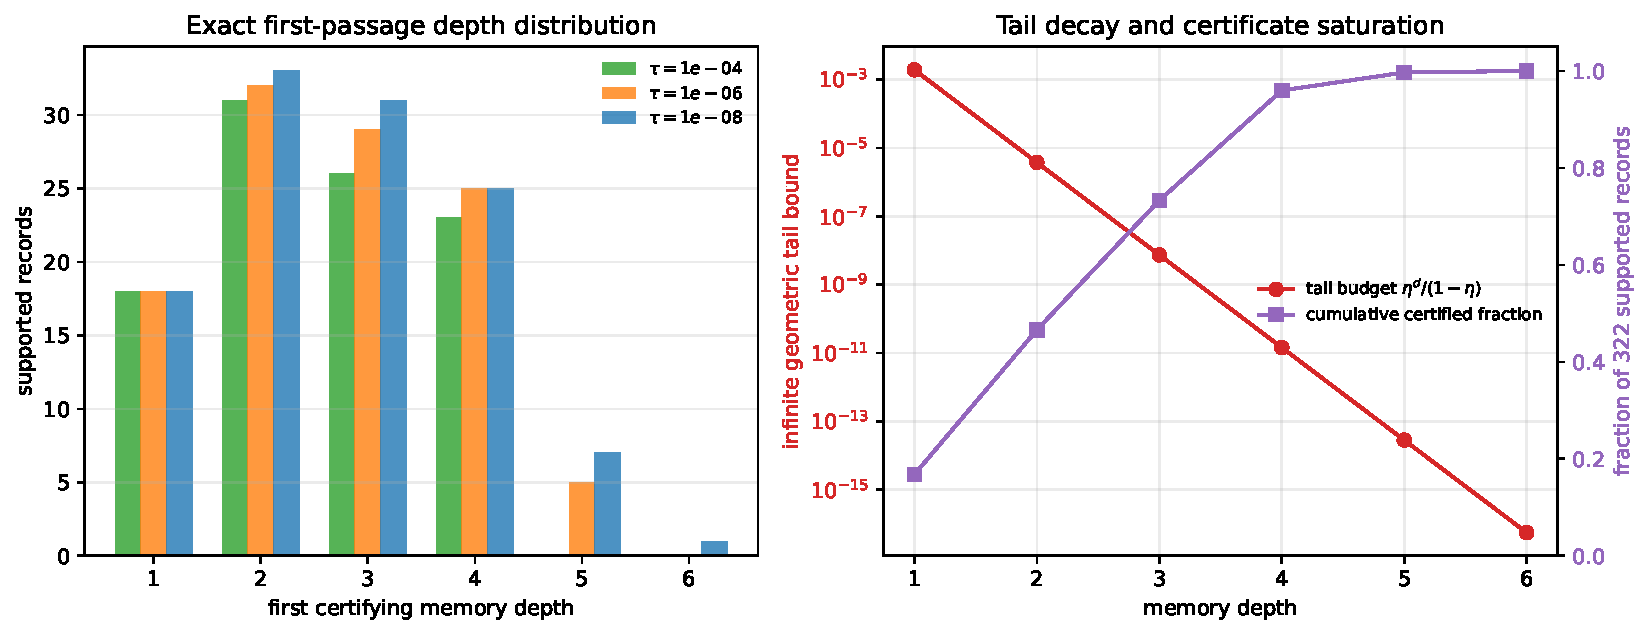
\includegraphics[width=\textwidth]{figures/monotone_memory_depth_optimization.pdf}
\caption{Left: exact first-passage depths.  Right: geometric tail decay and
cumulative saturation of the 322 supported records.}
\end{figure}

\section{Consequence and boundary}
The theoretical gain is the monotone first-passage principle: memory depth
is now an exactly optimizable certificate parameter, not a heuristic tuning
choice.  The numerical gain is that one consistent assembly recovers every
supported archived record, including the two weak $10^{-8}$ records not
closed by the fixed-depth RH-110 audit.

The largest observed depth six is not promoted to an all-level theorem.
Doing so would require physical lower margins and scale laws that persist
beyond the five anchors.  RH-117 therefore audits those scale trends and
proves what finite anchor data cannot imply.  Nothing here constructs a
Hilbert--Polya operator, identifies zeta zeros, closes uniform Stage A, or
proves the Riemann Hypothesis.

\bibliographystyle{plainnat}
\bibliography{references}
\end{document}
